\section{画像処理}

\markright{\arabic{section}. 画像処理}
画像処理の諸機能は,{\tt "vision/piximage"}ファイルに格納されている。
画像データを表現するために2つのクラス
{\bf pixel-image}と{\bf color-pixel-image}が定義されている。
ルックアップテーブル(LUT)を用いたピクセル(pixel)毎の変換,
エッジ抽出,pbmファイルへの画像データの変換が実現されている。

\subsection{ルックアップテーブル (LUT)}
LUTは,ピクセル(pixel)データを変換するためのベクトルデータである。 

\begin{refdesc}

\funcdesc{make-equilevel-lut}{levels \&optional (size 256)}{
1次元の整数ベクトル(integer-vector)を返す。
そのベクトルは,0から{\em size}までの値を0から{\em levels}までの値に
線形的にマップする。
例えば,{\tt (make-equilevel-lut 3 12)}は,
{\tt \#i(0 0 0 0 1 1 1 1 2 2 2 2)}を返す。}

\funcdesc{look-up}{src dest lut}{
ルックアップテーブル{\em lut}を用いて{\em src}ベクトルを{\em dest}ベクトルに
値を変換して置き換える。 もし{\em dest}ベクトルがNILのときは,
{\em src}ベクトルと同じクラスで同じサイズのベクトルを作る。
例えば, {\tt (look-up \#i(1 2 3) nil \#(10 20 30 40 50))}は,
{\tt \#i(20 30 40)}を返す。}

\funcdesc{look-up2}{src dest lut1 lut2}{
{\bf look-up2}は、ルックアップテーブル{\em lut1}および{\em lut2}を連続的に使用して
{\em src}ベクトルを{\em dest}ベクトルに変換する。
{\em src}と{\rm dest}は、同じサイズの整数ベクトルあるいはバイトベクトル(文字列)である。}


\funcdesc{look-up*}{src dest luts}{
{\em luts}は,ルックアップテーブルのリストである。
{\em luts}から与えられるルックアップテーブルを連続的に使用して,
{\em src}ベクトルを{\em dest}ベクトルに変換する。}

\funcdesc{concatenate-lut}{lut1 lut2 \&optional (size 256)}{
2つのルックアップテーブル{\em lut1}と{\em lut2}をつないだ
新しいルックアップテーブルを返す。その新しいテーブルを使用することは,
{\em lut1}と{\em lut2}を連続的に使用することと同じである。}

\funcdesc{make-colors}{default-color-map}{
以下に示すデフォルトのカラーマップを作る。}

\vardesc{*x-gray32-lut*}{
デフォルトカラーマップ{\tt x:*colormap*}
に定義されている32階調のグレースケールのLUTである。
{\tt (aref *x-gray32-lut* n)}は,32階調の内のn番目のグレー階調を返す。}

\vardesc{*x-gray16-lut*}{
デフォルトカラーマップ{\tt x:*colormap*}
に定義されている16階調のグレースケールのLUTである。}

\vardesc{*x-color-lut*}{
デフォルトカラーマップ{\tt x:*colormap*}
に定義されている幾つかの鮮明なカラーのLUTである。
登録されているカラーは, "black", "red", "green", "lightblue", "yellow",
"orange", "blue", "magenta", "white"である。}

\vardesc{*256to8*}{
0..255の範囲の整数を0..7の範囲に変換する256入力のLUTである。
その階調は,線形にマップされている。}

\vardesc{*256to16*}{
0..255の範囲の整数を0..15の範囲に変換する256入力のLUTである。
その階調は,線形にマップされている。}

\vardesc{*256to32*}{
0..255の範囲の整数を0..31の範囲に変換する256入力のLUTである。
その階調は,線形にマップされている。}

\vardesc{*gray32*}{
グレースケールピクセルをXのカラーマップに変換するための256入力のLUTである。
これは、{\tt *256to32*}と{\tt *x-gray32-lut*}を連結して作られる。
グレー32階調のXwindowの表示可能なピクセル画像は{\bf *gray32*}によって
グレー256階調の画像を変換することにより得ることができる。}

\vardesc{*rainbow32*}{
256階調のhue値をXのレインボーカラーマップに変換する
ための256入力のLUTである。
これは、{\tt *256to32*}と{\tt *x-rainbow32-lut*}を連結して作られる。}

\end{refdesc}

\subsection{ピクセル画像}
1枚の画像データは、{\bf pixel-image}クラスで表現される。{\bf pixel-image}は、
バイト型データを要素とする2次元配列である。それぞれのデータの内容は、
アプリケーションに依存している。一般的にピクセルの明るさを表現するために
使われるが、エッジ輝度や微分方向やカラー輝度やbarグラフのようなものにも用いることができる。

\begin{refdesc}
\classdesc{pixel-image}{array}{xpicture display-lut histogram\\
\>brightness-distribution0\\
\>brightness-distribution1\\
\>brightness-covariance}{
%provides a way to define image data with their horizontal/vertical sizes.
{\bf pixel-image}は、xwindowへの表示機能を持つ2次元の行列である。
pixelの変換は、{\bf display-lut}によって実現され、
その結果の画像は{\em xpicture}に蓄積される。
主な軸は縦方向にとる。{\tt (x,y)}の{\tt img}のピクセルは
{\tt (aref img y x)}でアクセスすることができる。}

\methoddesc{:width}{}{ピクセル画像の横サイズを返す。}
\methoddesc{:height}{}{ピクセル画像の縦サイズを返す。}
\methoddesc{:size}{}{配列の大きさを返す。}
\methoddesc{:transpose}{
\&optional (result (instance (class self) :init dim0 dim1))}{
x軸とy軸を交換する。}
\methoddesc{:map-picture}{lut \&optional (result (send self :duplicate))}{
この画像を{\em lut}で変換し、その画像データを{\em result}に蓄積する。}
\methoddesc{:map}{fn \&optional (result (send self :duplicate))}{
この画像のすべてのピクセルに{\em fn}を適用して、
{\em result}のピクセルに置く。}
\methoddesc{:brightest-pixel}{}{この画像の一番明るいピクセル値を見つける。}
\methoddesc{:darkest-pixel}{}{この画像の一番暗いピクセル値を見つける。}
\methoddesc{:average-pixel}{}{
この画像のすべてのピクセルの平均輝度を計算する。}
\methoddesc{:halve}{\&optional simage}{
半分の大きさの画像に縮小したピクセル画像を返す。}
% (:expand (rate) )
\methoddesc{:subimage}{x y subwidth subheight}{
この画像に{\em (x,y)}を左上角とし、幅が{\em subwidth}で高さが{\em subheight}
である四角形を切り出す。
その画像の原点は{\em (x,y)}に置かれる。
{\tt :subimage}は、この四角形で囲まれた画像を表現するピクセル画像を作る。}
\methoddesc{:xpicture}{\&optional lut}{
この画像を{\em lut}を用いて変換し、{\tt xpicture}に設定する。}
\methoddesc{:display-lut}{\&optional newlut}{
{\tt display-lut}にルックアップテーブル{\em newlut}を設定する。
その後、このルックアップテーブルを用いて画像を変換し、
{\tt xpicture}に設定する。}
\methoddesc{:display}{(xwin geometry:*viewsurface*)}{
{\bf :putimage}を用いて{\em xwin}で指定されるXwindowにこの画像を
表示する。
それぞれのピクセル値はXのカラーマップを参照する。
希望する表現を得るためには、このピクセル画像を固有のLUTで
変換すべきである。}
\methoddesc{:duplicate}{}{
この画像オブジェクトと同じ幅と高さを持つ同じクラスの
インスタンスを作る。ピクセルデータはコピーされない。}
\methoddesc{:copy-from}{src}{
{\em src}で指定される他の画像からピクセルデータをコピーする。
{\em src}とこの画像は同一の次元でなければならない。}
\methoddesc{:hex}{\&optional (x 0) (y 0) (w 16) (h 16) (strm t)}{
四角領域で示されるピクセルデータを16進数フォーマットで表示する。}
\methoddesc{:hex1}{\&optional (x 0) (y 0) (w 64) (h 16) (strm t)}{
四角領域で示されるピクセルデータを16進数フォーマットで表示する。}
\methoddesc{:prin1}{strm \&rest msg}{
このピクセル画像を名前と次元とともに表示する。}
\methoddesc{:init}{w h \&optional imgvec}{
幅{\em w}、高さ{\em h}を持つピクセル画像を初期化する。
%もし、すべてのピクセル値が文字列ベクトルで表現されている{\em imgvec}
%が与えられたとき、その長さは{\em w*h}でなければならない。
}
\methoddesc{:amplify}{rate \&optional (result (send self :duplicate)}{
{\em rate}をそれぞれのピクセル値に掛ける。}
\methoddesc{:compress-gray-scale}{levels \&optional result  \&aux pict2}{
この画像のピクセル値を0から{\em levels}までの範囲に変換をし、
その変換された画像を返す。}
\methoddesc{:lut}{lut1 \&optional (result (send self :duplicate))}{
ルックアップテーブル{\em lut1}を用いてこの画像を変換し、
その変換された画像を返す。}
\methoddesc{:lut2}{lut1 lut2 \&optional (result (send self :duplicate))}{
{\em lut1}と{\em lut2}を連結したルックアップテーブルを用いてこの画像を
変換し、その変換された画像を返す。}
\methoddesc{:histogram}{}{
この画像のそれぞれのピクセル値の発生回数を数え、そのヒストグラム
を整数ベクトル表現で返す。}
\methoddesc{:brightness-distribution}{}{
明るさの分散を返す。}
\methoddesc{:optimum-threshold}{}{
この画像の明るさの分散値が最大となっている階調を返す。}
\methoddesc{:project-x}{}{
同じx座標のピクセル値をすべて加算し、これらの値のベクトルを返す。}
\methoddesc{:project-y}{}{
同じy座標のピクセル値をすべて加算し、これらの値のベクトルを返す。}
\methoddesc{:digitize}{threshold \&optional (val0 0) (val1 255) result}{
{\em threshold}を用いてこの画像を{\em val0}と{\em val1}の2値画像に
変換する。}
\methoddesc{:and}{img2}{
この画像と{\em img2}のビット論理積をとり、処理した画像を返す。}
\methoddesc{:plot}{min max \&optional color viewsurface}{
{\em min}と{\em max}の間の値を持つピクセルをすべて{\em color}(gc)
で{\em viewsurface}にプロットする。}

%\longdescription{:edge1}{\&optional \= (method 1) \hspace{97mm} [メソッド]\\
\longdescription{:edge1}{\&optional \= (method 1) \` [メソッド]\\
\> (th1 *edge-intensity-threshold*) (th2 *weak-edge-threshold*)\\
\> (run *edge-length-threshold*)\\
\> (win geometry:*viewsurface*) (edgeimg1)}{
この画像のエッジを抽出し、Xwindow上にエッジ画像を表示する。}
\end{refdesc}

\subsection{カラーピクセル画像}
カラー画像は、{\bf color-pixel-image}クラスで表現される。
このクラスは、3つの{\bf pixel-image}を持っており、RGB表現の
red,green,blueあるいはHLSモデルの色合い,明るさ,濃さをそれぞれ表現する。
RGBとHLS間の変換もサポートしている。
\begin{refdesc}

\classdesc{color-pixel-image}{propertied-object}
{width height component1 component2 component3}{
3つの{\tt pixel-image}オブジェクトでカラー画像を表現する。}

\methoddesc{:width}{}{この画像の幅を返す。}
\methoddesc{:height}{}{この画像の高さを返す。}
\methoddesc{:size}{}{この画像の幅$\times$高さを返す。}
\methoddesc{:red}{}{{\tt component1}を返す。}
\methoddesc{:green}{}{{\tt component2}を返す。}
\methoddesc{:blue}{}{{\tt component3}を返す。}
\methoddesc{:hue}{}{{\tt component1}を返す。
色合い(hue)の値(0〜360)は、0〜255の1バイトで表現される。}
\methoddesc{:lightness}{}{{\tt component2}を返す。
正規化された明るさ(brightness)の値(0〜1)は、0〜255の整数で表現される。}
\methoddesc{:saturation}{}{{\tt component3}返す。
正規化された濃さ(saturation)の値(0〜1)は、0〜255の整数で表現される。}
\methoddesc{:pixel}{x y}{{\em (x,y)}における
{\tt component1,component2,component3}の値を3つの整数のリストとして返す。
このリストは、RGB値あるいはHLS値のどちらでも解釈できる。}
\methoddesc{:monochromize}{\&optional (NTSC nil)}{
RGB構成から明るさを計算し、新しい{\tt pixel-image}を返す。
もし、{\em NTSC}がNILなら、{\tt (R+G+B)/3}が計算される。
もし、Tなら、{\tt 0.299*R+0.587*G+0.114*B}が計算される。}
\methoddesc{:HLS}{}{この画像をRGB画像と仮定し、HLS表現に画像を変換する。
それぞれのピクセルを変換するために{\bf RGB2HLS}を呼び出す。}
\methoddesc{:RGB}{}{この画像をHLS画像と仮定し、RGB表現に画像を変換する。
それぞれのピクセルを変換するために{\bf HLS2RGB}を呼び出す。}
\methoddesc{:halve}{}{
この画像を半分のサイズに縮小した{\bf color-pixel-image}を返す。}
\methoddesc{:display}{\&optional (win *color-viewer*)}{
{\bf :putimage}を用いて{\em win}で指定されるXwindowに
このカラー画像を表示する。
それぞれのピクセル値はXのカラーマップを参照する。
希望する表現を得るためには、この画像を固有のLUTで
変換すべきである。}
\methoddesc{:display-lut}{\&optional (newlut1) (newlut2 newlut1) (newlut3 newlut2)}{
ルックアップテーブル{\em newlut1},{\em newlut2},{\em newlut3}を
{\tt display-lut}にそれぞれ設定する。それから、このルックアップテーブルを
使ってこの画像を変換し、{\tt xpicture}に設定する。}
%\longdescription{:edge1}{\&optional \= (method 1) \hspace{97mm} [メソッド]\\
\longdescription{:edge1}{\&optional \= (method 1) \` [メソッド]\\
\> (th1 *edge-intensity-threshold*) (th2 *weak-edge-threshold*)\\
\> (run *edge-length-threshold*)\\
\> (win *color-viewer*)}{
この画像のエッジを抽出する。Xwindow上にこのエッジ画像を表示する。}
\methoddesc{:hex}{\&optional (x 0) (y 0) (w 16) (h 16) (strm t)}{
四角領域で指定されるピクセルデータを16進数フォーマットで表示する。}
\methoddesc{:hex1}{\&optional (x 0) (y 0) (w 64) (h 16) (strm t)}{
四角領域で指定されるピクセルデータを16進数フォーマットで表示する。}
\methoddesc{:prin1}{strm \&rest msg}{
この画像を名前と次元と一緒に表示する。}
\methoddesc{:init}{width height \&optional r g b}{
カラー画像のサイズを定義し、{\tt pixel-image}にそれぞれカラーの1構成
を割り当てる。}
\end{refdesc}

ppmファイルがあったとき、次のプログラムでカラー値を画像に展開し、
Xwindowに表示をすることができる。
\begin{quote}
\begin{verbatim}
(setq ppmimg (read-pnm "xxx.ppm"))
(send ppmimg :hls)   ; RGB to HLS conversion
(make-ximage (send ppmimg :hue) *rainbow32*)
\end{verbatim}
\end{quote}

\subsection{エッジ抽出}
エッジ抽出機能は、{\tt "vision/edge/edge"}に実現されている。

\begin{refdesc}
%\longdescription{edge1}{img \= \&optional \= (method 1) \hspace{95mm} [関数]\\
\longdescription{edge1}{img \= \&optional \= (method 1) \` [関数]\\
\> \> (th1 *edge-intensity-threshold*)\\
\> \> (th2 *weak-edge-threshold*) \\
\> \> (run *edge-length-threshold*)\\
\> \> result\\
\> \&aux (width (send img :width)) (height (send img :height))}{
{\em img}のエッジピクセルを抽出する。
{\bf edge1}は、まずすべてのピクセルに微分オペレータを適用する。
次の3つの微分オペレータが用意されている。
{\bf grad3}は、縦と横の隣接ピクセルの差を用いる。
{\bf prewitt}は、{\bf grad3}に斜め方向のピクセルを考慮したものである。
{\bf sobel}は、{\bf prewitt}において横と縦のピクセルに重みを付けて差を計算したものを用いる。
{\em method}が0,1のとき{\bf grad3}、2のとき{\bf prewitt}、3のとき
{\bf sobel}を選択する。
{\em th1}より大きな輝度を持つエッジピクセルが強いエッジピクセルとして
指示される。
薄いエッジはエッジの輝度と微分方向を参照した後、独立したピクセルに付けられる。
これらの強いエッジの端から、強いエッジの方向に含まれる弱いエッジを捜し、
線分を延長する。
{\em th2}より大きなエッジ輝度を持つ弱いエッジは、無条件に繋げられる。
また、{\em th2}より小さなエッジ輝度を持つかなり弱いエッジは、他のエッジ
との距離が{\em run}以内であれば繋げられる。
{\bf edge1}は、強いエッジピクセルを1、弱いエッジあるいは
延長されたエッジピクセルを2、孤立したピクセルを255と表現する
{\bf pixel-image}オブジェクトを返す。}

\funcdesc{overlay-edge}{ximg edgeimg}{
Xwindowに表示可能な{\bf pixel-image}である{\em ximg}の最上位に
{\bf edge1}で得られた{\em edgeimg}を表示する。
強いエッジピクセルは赤、弱いエッジピクセルは緑、孤立したピクセルを青
で表現される。}

%\longdescription{edge2}{img1 edge1result \&key \= (:kvalue 8.0) \hspace{83mm} [関数]\\
\longdescription{edge2}{img1 edge1result \&key \= (:kvalue 8.0) \` [関数]\\
\> (:curve-threshold 0.8)\\
\> (:line-error 2.8)\\
\> (:curve-error 2.8)\\
\> (:plane-limit 0.3)}{
{\em edge1}の結果から一致する直線あるいは楕円曲線を捜す。
領域(region)、境界(boundary)、線分(line segment)の3つの要素の
リストが返される。}

\end{refdesc}

{\bf edge2}で出力される3つの要素は、以下のように定義される。

\begin{refdesc}
\classdesc{region}{propertied-object}{contour area intensity std-deviation}{
領域を表現。}
\classdesc{boundary}{propertied-object}{parent-region
		hole
		segments
		intensity
		topleft
		bottomright
		length}{
境界を表現。}
\classdesc{edge-segment}{propertied-object}{prev next 
		wing	; the other half-edge
		intensity std-deviation 
		start end}{
エッジ線分を表現。}
\classdesc{line-edge-segment}{edge-segment}{la lb}{
直線のエッジ線分を表現。}
\classdesc{curved-edge-segment}{edge-segment}{rotation total-rot side
			a b c d e}{
曲線のエッジ線分を表現。}

\funcdesc{draw-ellipse-segment}{elp gc \&optional (vs *viewsurface*)
				      (height (send vs :height))
					(x 0) (y 0)}{
{\em vs}で指定されるXwindowに{\bf curved-edge-segment}オブジェクトである
{\em elp}を描く。}
\funcdesc{draw-line-segment}{s \&optional gc (vs *viewsurface*)
				(height (send vs :height))
				(x 0) (y 0)}{
{\em vs}で指定されるXwindowに{\bf line-edge-segment}オブジェクトである
{\em s}を描く。}
%\longdescription{draw-segments}{segs \&key \= (:line-gc image::*red-gc*) \hspace{67mm} [関数]\\
\longdescription{draw-segments}{segs \&key \= (:line-gc image::*red-gc*) \` [関数]\\
\> (:ellipse-gc line-gc)\\
\> (:vs geometry:*viewsurface*)\\
\> (:height (send vs :height))\\
\> (:step nil)\\
\> (:x 0) (:y 0)}{
{\em vs}で指定されるXwindowに{\bf edge-segment}のリスト表現である
{\em segs}を描く。}
\funcdesc{draw-boundary}{b \&optional gc}{
{\em vs}で指定されるXwindowに{\bf boundary}のオブジェクト{\em b}
の中の線分を描く。}
\funcdesc{draw-boundaries}{bs \&optional gc (step nil)}{
{\em vs}で指定されるXwindowに{\bf boundary}のリスト表現である{\em bs}
の中の線分を描く。}

\vardesc{*red-gc*}{\#ff0000(赤色)の色を持つ{\bf gcontext}。}
\vardesc{*blue-gc*}{\#0000ff(青色)の色を持つ{\bf gcontext}。}
\vardesc{*green-gc*}{\#00ff00(緑色)の色を持つ{\bf gcontext}。}
\vardesc{*yellow-gc*}{\#ffff00(黄色)の色を持つ{\bf gcontext}。}
\vardesc{*cyan-gc*}{\#00ffff(水色)の色を持つ{\bf gcontext}。}

\end{refdesc}

\begin{figure}
\begin{center}
% \epsfile{file=fig/corri30.ps,height=10cm}
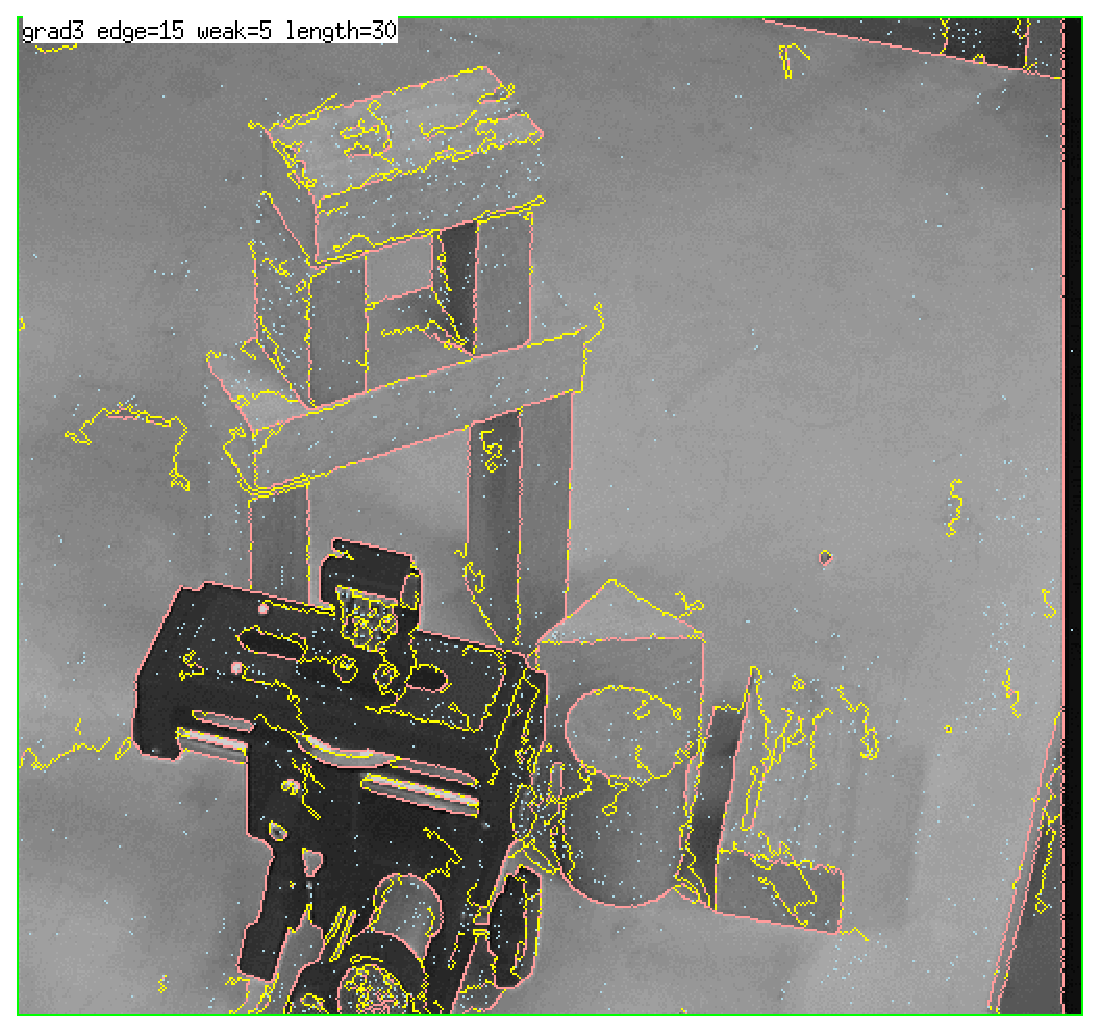
\includegraphics[height=9cm]{fig/block1.edg.ps}
%\epsfile{file=fig/block1.edg.ps,height=9cm}
\caption{Edge Finder and Overlaied Edges}
\end{center}
\end{figure}

\subsection{\label{tracking}トラッキング}
{\tt "vision/correlation"}に元画像とトラッキングしたい画像との
相関を求める関数が定義されている。

\begin{refdesc}
\classdesc{tracking-window}{pixel-image}{x-pos y-pos x-vel y-vel\\
\>pattern-size window-size\\
\>x-win y-win window window-margin\\
\>update threshold half-pattern correlation}{
このクラスは、トラッキング画像を定義する。}

\methoddesc{:correlation}{}{
この画像と元画像との間の相関を返す。}
\methoddesc{:grab}{\&optional (x x-pos) (y y-pos) (sampling 2)}{
画像入力装置から画像を取り込み、その画像の{\bf pixel-image}を返す。}
\methoddesc{:window-rectangle}{val}{
Xwindowの上に四角形を描く。}
\methoddesc{:rectangle}{val}{
Xwindowの上に四角形を描く。}
\methoddesc{:move}{newpos \&aux (newx (aref newpos 0)) (newy (aref newpos 1))}{
トラッキングする位置を{\em newpos}に移動し、新しい画像を取り込む。}
\methoddesc{:track}{display-window \&optional th}{
Xwindowの画像からこの画像をトラッキングする。}
\methoddesc{:serach}{display-window \&optional th}{
Xwindowの画像からこの画像を捜す。}
\methoddesc{:track-and-search}{flag \&optional th}{
この画像をトラッキングする。
もし、トラッキングを失敗したとき、Xwindowからこの画像を捜して
位置を更新する。}

\methoddesc{:pos}{}{
windowの左上位置を返す。}
\methoddesc{:vel}{}{
トラッキング速度を返す。}
\methoddesc{:insidep}{pos \&aux (x (aref pos 0)) (y (aref pos 1))}{
{\em pos}が{\bf tracking-window}の中に含まれるかどうかをチェックする。}
\methoddesc{:update}{\&optional (flag :get)}{
{\tt update}に{\em flag}を設定する。もし、{\em flag}がなければ、
{\tt update}を返す。}
\methoddesc{:prin1}{strm \&rest mesg}{
この{\bf tracking-window}を名前と次元と一緒に表示する。}
\methoddesc{:init}{x y size win-size}{
{\bf tracking-window}を作成する}
\end{refdesc}

\subsection{\label{PBMfile}画像ファイル入出力}
%There are lots of file formats defined for the representation of
%pixel images.
{\tt "vision/pbmfile"}は、Euslispとディスクファイルとの間の
画像データを変換する関数を定義している。
EusLispは、pgm(portable gray-scale map)とppm(portable pixmap)フォーマット
のファイルの読み書きができる。

\begin{refdesc}
\funcdesc{read-pnm}{f \&optional buf0 buf1 buf2}{
{\bf file-stream}の{\em f}で指定されるpgmあるいはppmファイル
を読み込み、{\bf pixel-image}あるいは{\bf color-pixel-image}を返す。
画像ファイルは、asciiでもバイナリーでも可能である。
言い換えれば、P2,P3,P5,P6フォーマットは認識できる。}
\funcdesc{read-pnm-file}{file \&optional buf0 buf1 buf2}{
ファイル名{\em file}で指定されるpgmあるいはppmファイルを読み込む。
%この関数は、{\bf read-ppm}を呼び出す。
}

\funcdesc{write-pgm}{f image  \&optional (depth 255)}{
{\em image}で指定される{\bf pixel-image}を{\bf file-stream}である{\em f}
にバイナリーppmフォーマットで書き込む。
%(この関数は、コメントを追加することで変更できる。)
}
\funcdesc{write-ppm}{f image  \&optional (depth 255)}{
{\em image}で指定される{\bf pixel-image}を{\bf file-stream}である{\em f}
にバイナリーpgmフォーマットで書き込む。}
\funcdesc{write-pnm}{f img}{
{\em img}で指定されるピクセル画像を{\bf file-stream}である{\em f}に書き込む。
もし、{\em img}が{\bf pixel-image}であるなら、バイナリーpgmフォーマットで
書き込み、{\bf color-pixel-image}ならバイナリーppmフォーマットで書き込む。}
\funcdesc{write-pnm-file}{file img}{
ファイル名{\em file}に{\em img}で指定されるピクセル画像を書き込む。
この関数は、{\bf write-pnm}を呼び出す。}

\funcdesc{image::read-raw-image}{file \&optional (x 256) (y x)}{
raw-imageファイルを読み込み、1次元の文字列ベクトルを返す。
%座標系についてなにも前提がない。
raw-imageの次元は、与えられた{\em x}と{\em y}に一致しなければならない。}
\funcdesc{image::write-raw-image}{file imgvec}{
ピクセル値を1バイトのベクトル(文字列)に蓄積した{\em imgvec}を{\em file}
に書き込む。}
\end{refdesc}

\newpage
